\documentclass{article}

\usepackage[utf8]{inputenc}
\usepackage[T1]{fontenc}
\usepackage{lipsum}
\usepackage{graphicx}
\usepackage{amsmath}
\usepackage[margin=1in]{geometry}
\usepackage{titlesec}

\titleformat{\section}
{\LARGE\bfseries}{\thesection}{1em}{}

\titleformat{\subsection}
{\Large\bfseries}{\thesection}{1em}{}

\begin{document}

\pagestyle{empty}

\section*{Use case}
\large
\subsection*{Introduzione}
Obiettivi:
\begin{enumerate}
    \renewcommand{\labelenumi}{-}
    \itemsep0em
    \item Identificare i \textit{casi d'uso}
    \item Connettere i casi d'uso rispetto agli obiettivi dell'\textit{attore principale}
    \item Mantenere uno stile \textit{essenziale}, non troppo informativo, poichè potrebbe rendere maggiormente difficile l'individuazione del \textit{goal}
    \item Adottare uno \textit{sviluppo iterativo} 
\end{enumerate}
\textbf{Use case} spesso è indicato come il meccanismo per scoprire e registrare i requisiti, di carattere \textit{funzionale}. La scrittura dei \textit{casi d'uso} è un eccellente tecnica per capire e descrivere ciò che il \textit{sistema} debba implementare, rispetto ad una totalità di influenze esterne che creino la situazione ideale per poter proseguire con il compimento dell'obiettivo principale da parte del \textit{soggetto}.
\textbf{UP}, ossia \textit{Unified Process}, indica un certo modello dei casi d'uso, definito come \textbf{modello comportamentale}, per cui fortemente connesso rispetto ai \textit{comportamenti} degli elementi trattati.\vspace*{14pt}\\
I \textit{diagrammi} dei \textit{casi d'uso} sono \textbf{diagrammi comportamentali} utilizzati per descrivere un insieme di azioni, o meglio \textit{behavior}, che un sistema deve svolgere insieme ad uno o più utenti esterni al sistema. Inoltre, carattere imprescindibile di tale modellazione, prevede che ogni \textit{use case} fornisca un \textbf{risultato di valore}, per gli utenti con cui interagiscono oppure per gli \textit{stakeholders}. \textit{Customers} e \textit{final users} pongono certi obiettivi, detti \textit{needs}, i quali richiedono che \textit{sistemi} siano in grado di rendere chiaro il loro \textbf{connubio}.\vspace*{14pt}\\
Differenti sono gli approcci dettati, tuttavia le strategie migliori riguardano un uso semplice e famigliare degli strumenti messi a disposizione, poichè rendono più semplice la lettura del modello, contribuiscono alla ricerca dei requisiti necessari e abbassa il rischio di perdere l'obiettivo su cui fonda l'intera architettura, definito anche \textit{missing the mark}.\\
Infatti il primo step ricade nella comprensione del problema assieme all'individuazione dei requisiti funzionali che comporranno i casi d'uso, affinchè siano comprensibili da parte dei portatori di interesse. Tuttavia, quest'ultimo passaggio rappresenta la maggiore difficoltà di questo modello, ossia la decisione e scoperta di cosa sia potenzialmente necessario; durante una prima fase di analisi potrebbero essere inseriti dei \textit{layer sofistaticati-aggiuntivi}, i quali solitamente oscurano il reale proseguimento del \textit{mark}.\vspace*{14pt}\\
Per cui, ricapitolando, il diagramma dei casi d'uso è utilizzato per specificare:
\begin{enumerate}
    \renewcommand{\labelenumi}{-}
    \itemsep0em
    \item I requisiti esterni degli stakeholders, funzionali rispetto a quanto il sistema debba implementare
    \item Le funzionalità offerte dal sistema per tutti i final user esterni
    \item Rispettare i limiti secondo cui il sistema debba sottostare, defininendo come tale ambiente debba interagire con il soggetto pur di proseguire verso il \textit{path} voluto
\end{enumerate}

\subsection*{Elementi del diagramma}
In questa sezione si analizzano gli elementi comuni ad un qualsiasi diagramma dei casi d'uso, descrivendo successivamente caratteristiche uniche rispetto alle strategie elencate.\vspace*{14pt}\\
\textit{Definizione informale}\\
Un \textbf{attore} è qualcosa caratterizzato da un comportamento, come una persona, un computer system oppure un'organizzazione.\vspace*{14pt}\\
Per cui, descrivendone maggiormente il ruolo svolto, un \textbf{attore} è un \textbf{classificatore comportamentale}, ossia un'entità che interagisce con il sistema implementato o ideato mediante \textbf{interazioni}, quali, semplicemente, l'invio di segnali o di dati.\vspace*{14pt}\\
\textit{Definzione informale}\\
Uno \textbf{scenario}, definita anche \textit{istanza} del caso d'uso, indica un preciso percorso attraversando certi e specifici \textit{use case}.\vspace*{14pt}\\
Quindi il modello comportamentale trattato è definito mediante un insieme di scenari fallimentari o di successo, in relazione al conseguimento dell'obiettivo dell'attore principale, adeguandosi ai comportamenti illustrati all'interno dei singoli casi d'uso. E' bene sottolineare come ogni caso d'uso rappresenti uno specifico requisito funzionale, posto al di fuori del diagramma, dove solamente mediante interazioni è possibile stabilire un path per cui il sistema sia in grado di raggiungere l'obiettivo.\\
UP definisce differenti formati e tipi di use case...

\pagebreak
\begin{center}
    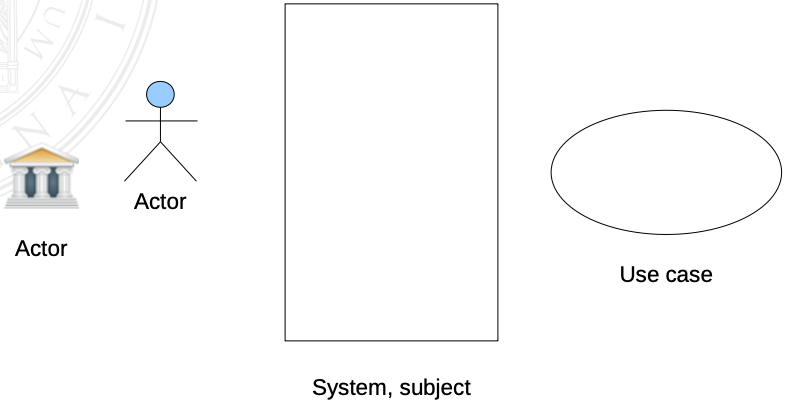
\includegraphics[width=0.7\textwidth]{foto 1.png}
\end{center}

\subsection*{Attore}
\large

Negli UML un \textbf{attore} è un \textbf{classificatore comportamentale} che \textit{specifica il ruolo svolto da un entità esterna che interagisce con il soggetto} (ad esempio, scambiando segnali e dati), un utente umano del sistema, altri sistemi o hardware che utilizza servizi del soggetto.

\subsection*{Soggetto}
\large

Il \textbf{soggetto} è il \textbf{sistema sotto analisi} al quale vengono applicati i diversi casi d'uso. Il soggetto può essere un business, un sistema software, un sistema fisico, o un sottosistema più piccolo con qualche comportamento. In termini di UML, il soggetto è un \textbf{classificatore di casi d'uso} che ha il ruolo di "\textit{soggetto}". \\ \\

\subsection*{Casi d'uso}
\large

Negli UML, un \textbf{caso d'uso} è un \textbf{classificatore comportamentale} che specifica il comportamento di un soggetto descrivendo una \textbf{sequenza di azioni} eseguite dal sistema per ottenere un \textbf{risultato osservabile} di un qualche valore per uno o più attori o stakeholders del sistema. Ogni caso d'uso quindi descrive un'unità di una funzionalità utile e finita che il soggetto fornisce agli utenti. Vengono di solito rappresentati graficamente come un \textbf{ellisse} contenente il nome del caso d'uso.

\subsection*{Relazioni tra attori}
\large

Possiamo definire attori astratti o reali e specializzarli usando \textbf{relazioni di generalizzazione}. La generalizzazione tra attori è rappresentata graficamente come una \textbf{linea direzionata da una grande punta} (stesso discorso per la generalizzazione tra classi).
\begin{center}
    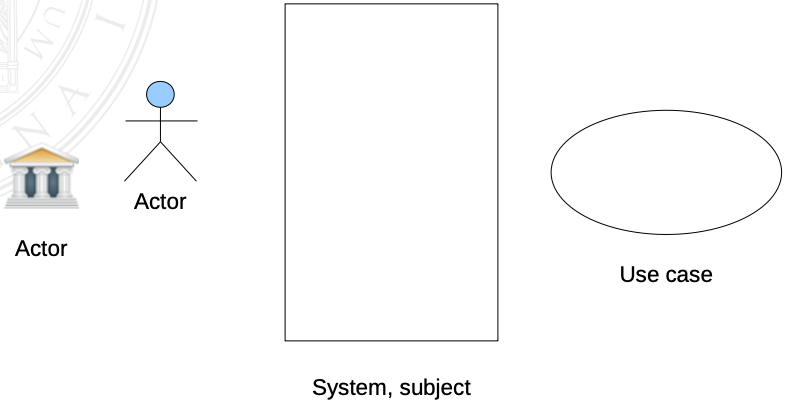
\includegraphics[width=0.4\textwidth]{foto 2.png}
\end{center}

\subsection*{Associazioni tra attori e casi d'uso}
\large

Ogni caso d'uso specifica delle funzionalità utili che il soggetto fornisce agli attori. Queste funzionalità devono essere \textbf{inizializzate da un attore}. Gli attori possono essere connessi ad un caso d'uso soltanto da una \textbf{associazione relazionale binaria}.
\begin{center}
    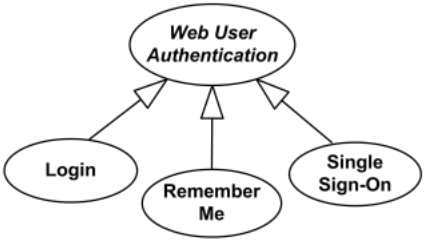
\includegraphics[width=0.4\textwidth]{foto 3.png}
\end{center}

\subsection*{Relazioni tra casi d'uso}
\large

I casi d'uso possono essere organizzati usando le seguenti relazioni:
\begin{enumerate}
    \renewcommand{\labelenumi}{-}
    \item \textbf{Generalizzazione}
    \item \textbf{Extend}
    \item \textbf{Include}
    \item (\textit{Associazione})
\end{enumerate}

\subsection*{Generalizzazione}
\large

La generalizzazione viene rappresentata graficamente come una \textbf{linea direzionata da una grande punta} (stesso discorso per la generalizzazione tra classi), dove la freccia va \textbf{dal caso più specifico verso quello più generico}.
\begin{center}
    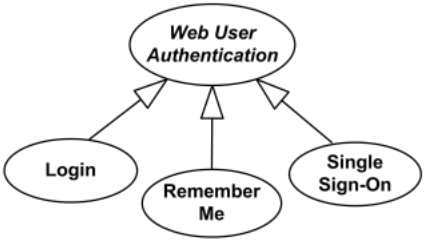
\includegraphics[width=0.4\textwidth]{foto 4.png}
\end{center}
In foto possiamo osservare diversi modi per eseguire il "Web User Authentication". Ogni modo porta allo stesso obiettivo, ma con \textbf{percorsi diversi}.

\subsection*{Extend}
\large

L'\textbf{extend} è una relazione diretta che specifica come e quando il comportamento definito in maniera opzionale, \textit{che estende il caso d'uso}, \textbf{può essere} inserito nel comportamento definito nel caso d'uso esteso. L'estensione prende luogo in uno o più punti di estensione definiti nel caso d'uso esteso. Le relazioni \textit{extend} vengono rappresentate graficamente come una \textbf{freccia tratteggiata con una punta aperta}, dove la freccia va \textbf{dal caso esteso verso il caso base}. La freccia viene inoltre rinominata con la \textbf{parola chiave "extend"}. \\ \\
Un \textbf{punto di estensione} è una funzionalità di un caso d'uso che \textbf{identifica un punto nel comportamento del caso d'uso dove il comportamento può essere esteso da altri casi d'uso}, come già specificato dalla relazione di estensione.
I punti di estensione possono essere rappresentati graficamente in \textbf{uno spazio del simbolo ovale dei casi d'uso}. Ogni punto di estensione deve avere un nome, unico all'interno del caso d'uso.
\begin{center}
    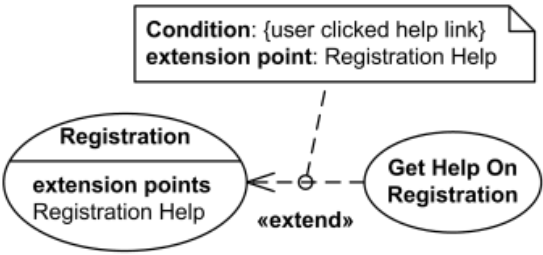
\includegraphics[width=0.4\textwidth]{foto 5.png}
\end{center}

\subsection*{Include}
\large

Una \textbf{relazione di inclusione} è una relazione diretta tra due o più casi d'uso utilizzata quando un comportamento richiesto,\textbf{ non opzionale}, è \textbf{inserito nei comportamenti inclusi nel caso d'uso base}. Questo tipo di relazione può essere usato quando:
\begin{enumerate}
    \renewcommand{\labelenumi}{-}
    \item ci sono parti comportamentali comuni tra due o più casi d'uso
    \item per semplificare grandi casi d'uso dividendolo in più casi d'uso
\end{enumerate}
Una relazione di inclusione può essere rappresentata graficamente come una \textbf{freccia tratteggiata con una punta aperta}, dove la freccia va \textbf{dal caso d'uso base verso il caso d'uso da includere} (comune per più casi d'uso). La freccia viene inoltre rinominata con la \textbf{parola chiave "include"}.
\begin{center}
    
\includegraphics[width=0.4\textwidth]{foto 6.png}
\end{center}

\subsection*{Esempio di diagramma dei casi d'uso}
\large
\begin{center}
    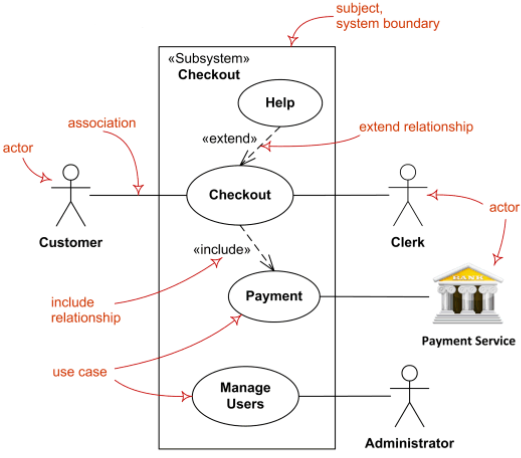
\includegraphics[width=0.8\textwidth]{foto 7.png}
\end{center}
\textit{Nota Bene}: è consuetudine, se è presente ambiguità su quale attore sia l'inizializzatore, che ad inizializzare sia l'attore di sinistra.

\subsection*{Casi d'uso di sistema vs casi d'uso business}
\large

L'obiettivo primario è di avere sempre un modello completo e preciso. Tuttavia, ci sono delle differenze tra i casi d'uso di sistema e i casi d'uso business. Il primo ha come soggetto il sistema, mentre il secondo un organizzazione. Inoltre, per i casi d'uso business, gli attori possono essere anche interni all'organizzazione.

\subsection*{Portata del caso d'uso di sistema}
\large

Per quanto riguarda la creazione di un caso d'uso, si cerca di creare il \textbf{più piccolo insieme di attività} che offre un risultato significativo per l'utente, definito da obiettivi che possono essere completati in una \textbf{sessione}. Di solito si tratta di una dozzina di passi. Quando un caso d'uso coinvolge più attori con obiettivi diversi si divide il caso d'uso in più casi d'uso.

\subsection*{Cosa fare e cosa non fare con i casi d'uso}
\large
\begin{enumerate}
    \renewcommand{\labelenumi}{-}
    \item Sommario visuale delle diverse funzionalità
    \item Evitare di specificare troppo i passaggi tramite interfaccia grafica (può essere modificata durante lo sviluppo)
    \item Non decomporre per altri motivi diversi dal riutilizzo
    \item Avere una comprensione accurata delle differenze tra generalizzazione, inclusione e estensione
    \item Non creare nuove relazione stereotipate
    \item Il tempo può essere un attore
    \item Gli attori sono esterni al sistema (per casi d'uso di sistema)
\end{enumerate}
Vediamo ora un esempio di due casi d'uso rappresentati graficamente. In quello di sinistra abbiamo una rappresentazione meno dettagliata, ma comunque efficace. A destra risulta essere molto informativa (anche troppo).
\begin{center}
    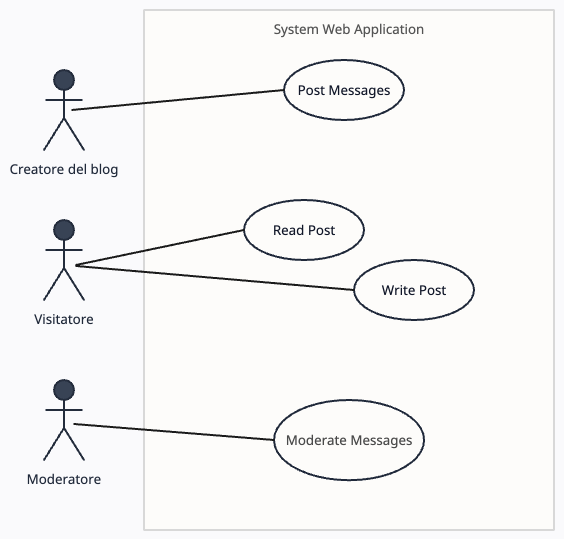
\includegraphics[width=1\textwidth]{foto 8.png}
\end{center}

\subsection*{Modello di casi d'uso e diagramma dei casi d'uso}
\large

Un diagramma UML per un caso d'uso \textbf{NON} è un modello di caso d'uso! Il diagramma può essere visto come un \textbf{sommario}, non avendo al suo interno aspetti fondamentali come i dettagli sulle fasi di interazione e quando il caso d'uso viene applicato, le condizioni pre/post, ecc. Inoltre, \textbf{non esiste} una notazione standard per rappresentare un modello di caso d'uso, ma esistono molti \textbf{template} utilizzati in base al caso specifico. I template possono essere \textbf{molto dettagliati o più semplici}, in base ai differenti casi e dal team di sviluppo (è fondamentale rimanere costanti). In ogni template sono presenti diverse \textbf{sequenze}, che ci indicano i diversi casi possibili durante una ipotetica esecuzione. Spesso, oltre alla sequenza che illustra l'esecuzione ottimale (\textit{Happy path}), vengono indicate sequenze alternative che portano comunque all'obiettivo finale seguendo un percorso diverso. Può anche esserci una sequenza (\textit{Exceptions}) dove non viene raggiunto l'obiettivo.

\subsection*{Sequenze}
\large

Il concetto di sequenza è presente in tutti i template per i modelli di caso d'uso. Vediamo un esempio di sequenza (vengono tralasciate le cose più ovvie, come le precondizioni):\\ \\
\textit{MAIN SUCCESS SEQUENCE (a.k.a. Happy path)}:
\begin{enumerate}
    \item L'utente seleziona l'opzione per entrare in un nuovo trasferimento
    \item Il sistema mostra il modulo per effettuare il trasferimento (conto destinatario, dettagli, importo, data)
    \item L'utente inserisce i dati nel modulo ed effettua l'ordine
    \item Il sistema mostra il messaggio di accettazione dell'ordine
\end{enumerate}
\textit{EXTENSIONS}:

3a. Importo non disponibile:

3a1. Il sistema mostra un messaggio di errore e torna allo step 2\\ \\
Vogliamo capire soltanto il caso d'uso, non come viene eseguito o come deve essere svolto ogni passaggio. Ci chiediamo quindi solo \textbf{cosa} vuole fare, e non \textbf{come} deve farlo!

\subsection*{Scenari}
\large

Uno scenario può essere visto come una instanza di un caso d'uso. Descrive una possibile interazione tra attori ed il sistema. Vengono utilizzati per documentazione e per creare casi di test.\\ \\
Usare uno scenario è molto utile per i casi di testing, dove possiamo spiegare gli ipotetici \textit{n} scenari possibili. Un altro motivo è che cerchiamo di catturare i requisiti funzionali del sistema. Usando uno scenario come test verifichiamo il funzionamento del caso d'uso.

\subsection*{Stati di un modello di caso d'uso}
\large

Un modello di casi d'uso è tendenzialmente soggetto a perfezionamenti iterativi (possiamo vederlo come una sorta di ciclo di vita del modello):
\begin{enumerate}
    \renewcommand{\labelenumi}{-}
    \item Obiettivo stabilito
    \item Struttura della storia compresa
    \item Storia più semplice completata
    \item Storia sufficiente completata
    \item Tutte le storie completate
\end{enumerate}

\subsection*{Esercizio}
\large
Un \textit{blog} è una \textit{web application} che contiene una serie di messaggi (\textit{post}) datati su diversi argomenti. I messaggi vengono postati dal creatore del blog che li mette online. L'autore può associare ad ogni messaggio una o più categorie (tramite delle parole chiave). \\
I visitatori del blog possono commentare i messaggi; i commenti, se approvati dal moderatore (di solito è il creatore del blog), appaiono in una sezione specifica sotto il messaggio originale. \\ \\
Partiamo capendo quale sia il soggetto, ovvero la nostra \textit{web application}. Procediamo poi trovando gli attori:
\begin{enumerate}
    \renewcommand{\labelenumi}{-}
    \item Creatore del blog
    \item Visitatore
    \item Moderatore
\end{enumerate}
L'obiettivo del creatore del blog è quello di \textbf{pubblicare i messaggi}.\\
Vediamo ora un modello di casi d'uso d'esempio per questo caso:
\begin{center}
    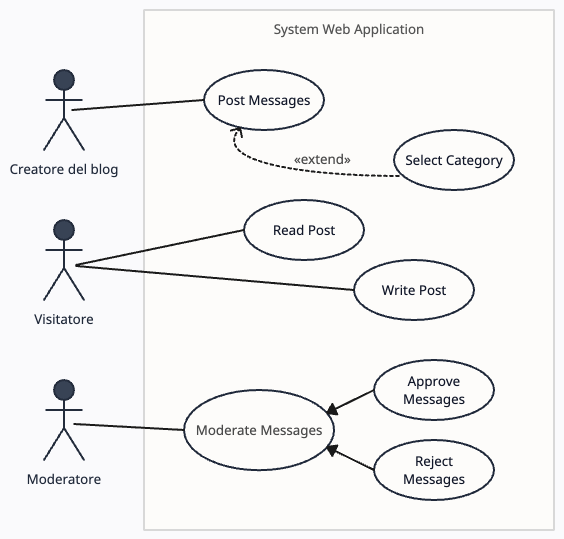
\includegraphics[width=0.6\textwidth]{foto 9.png}
\end{center}
Come possiamo osservare, abbiamo i nostri tre attori (creatore del blog, visitatore e moderatore) ed i loro obiettivi.
Un'altra possibile soluzione poteva essere la seguente:
\begin{center}
    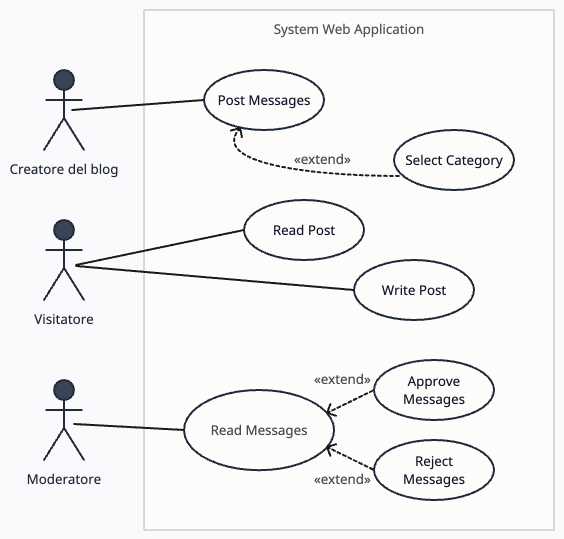
\includegraphics[width=0.6\textwidth]{foto 10.png}
\end{center}
In questo caso dovremmo specificare in qualche modo che non possono essere eseguite entrambe le operazioni (approve e reject), ma soltanto una per commento (magari tramite l'utilizzo di XOR). Tra i due approcci è preferibile il primo, non dovendo specificare l'esclusività e per un approccio meno confusionario rispetto al secondo.
Se volessimo mantenere un modello funzionale più semplice:
\begin{center}
    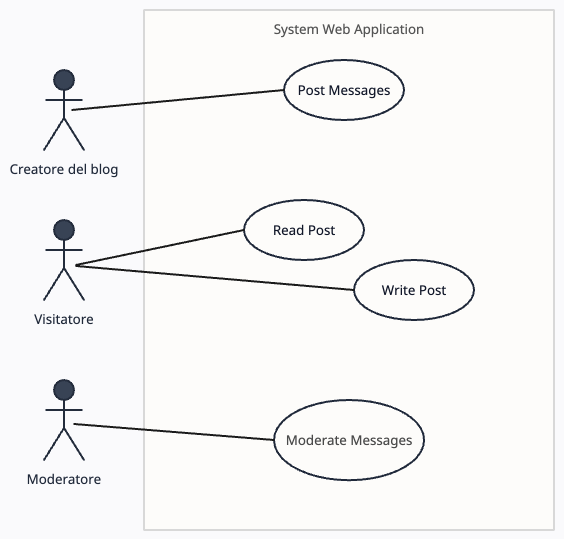
\includegraphics[width=0.6\textwidth]{foto 11.png}
\end{center}
Questa soluzione è buona, anche se meno dettagliata. In questo caso però il più completo è migliore, perchè non risulta essere troppo confusionario. Ripensando al ciclo di vita di un modello di casi d'uso, questa potrebbe essere la fase iniziale della modellazione.\\ \\
Se avessimo voluto usare un template di caso d'uso semplice, avremmo ottenuto (stiamo considerando l'obiettivo \textit{write comment}):
\begin{enumerate}
    \renewcommand{\labelenumi}{-}
    \item \textbf{UC1}: write comment
    \item \textbf{Actors}: visitor 
    \item \textbf{Pre-condition}: utente visualizza il messaggio
    \item \textbf{Main Sequence}:  
    \begin{enumerate}
        \item utente scrive il commento
        \item utente invia il commento
        \item sistema conferma la ricezione del commento
    \end{enumerate}
    \item \textbf{Alternative Sequence}: il messaggio contiene linguaggio non appropriato\\
    (c1) Il sistema cancella il commento
    \item \textbf{Post-condition}: il messaggio viene aggiunto alla lista dei messaggi da moderare
\end{enumerate}
\end{document}